% !TeX TS-program = xelatex

\documentclass{resume}
\ResumeName{向嘉豪}

% 如果想插入照片,请使用以下两个库。
\usepackage{graphicx}
\usepackage{tikz}

\setCJKmainfont{Kaiti SC}

\begin{document}

\ResumeContacts{
  (+86)130-8728-6239,%
  \ResumeUrl{mailto:jiahaoxiang2000@gmail.com}{jiahaoxiang2000@gmail.com},%
  \ResumeUrl{https://github.com/jiahaoxiang2000}{github.com/jiahaoxiang2000} \footnote{下划线内容包含超链接。}%
}

% 如果想插入照片,请取消此代码的注释。
% 但是默认不推荐插入照片,因为这不是简历的重点。
% 如果默认的照片插入格式不能满足你的需求,你可以尝试调整照片的大小,或者使用其他的插入照片的方法。
% 不然,也可以先渲染 PDF 简历,然后用其他工具在 PDF 上叠加照片。
\begin{tikzpicture}[remember picture, overlay]
  \node [anchor=north east, inner sep=1cm]  at (current page.north east)
  {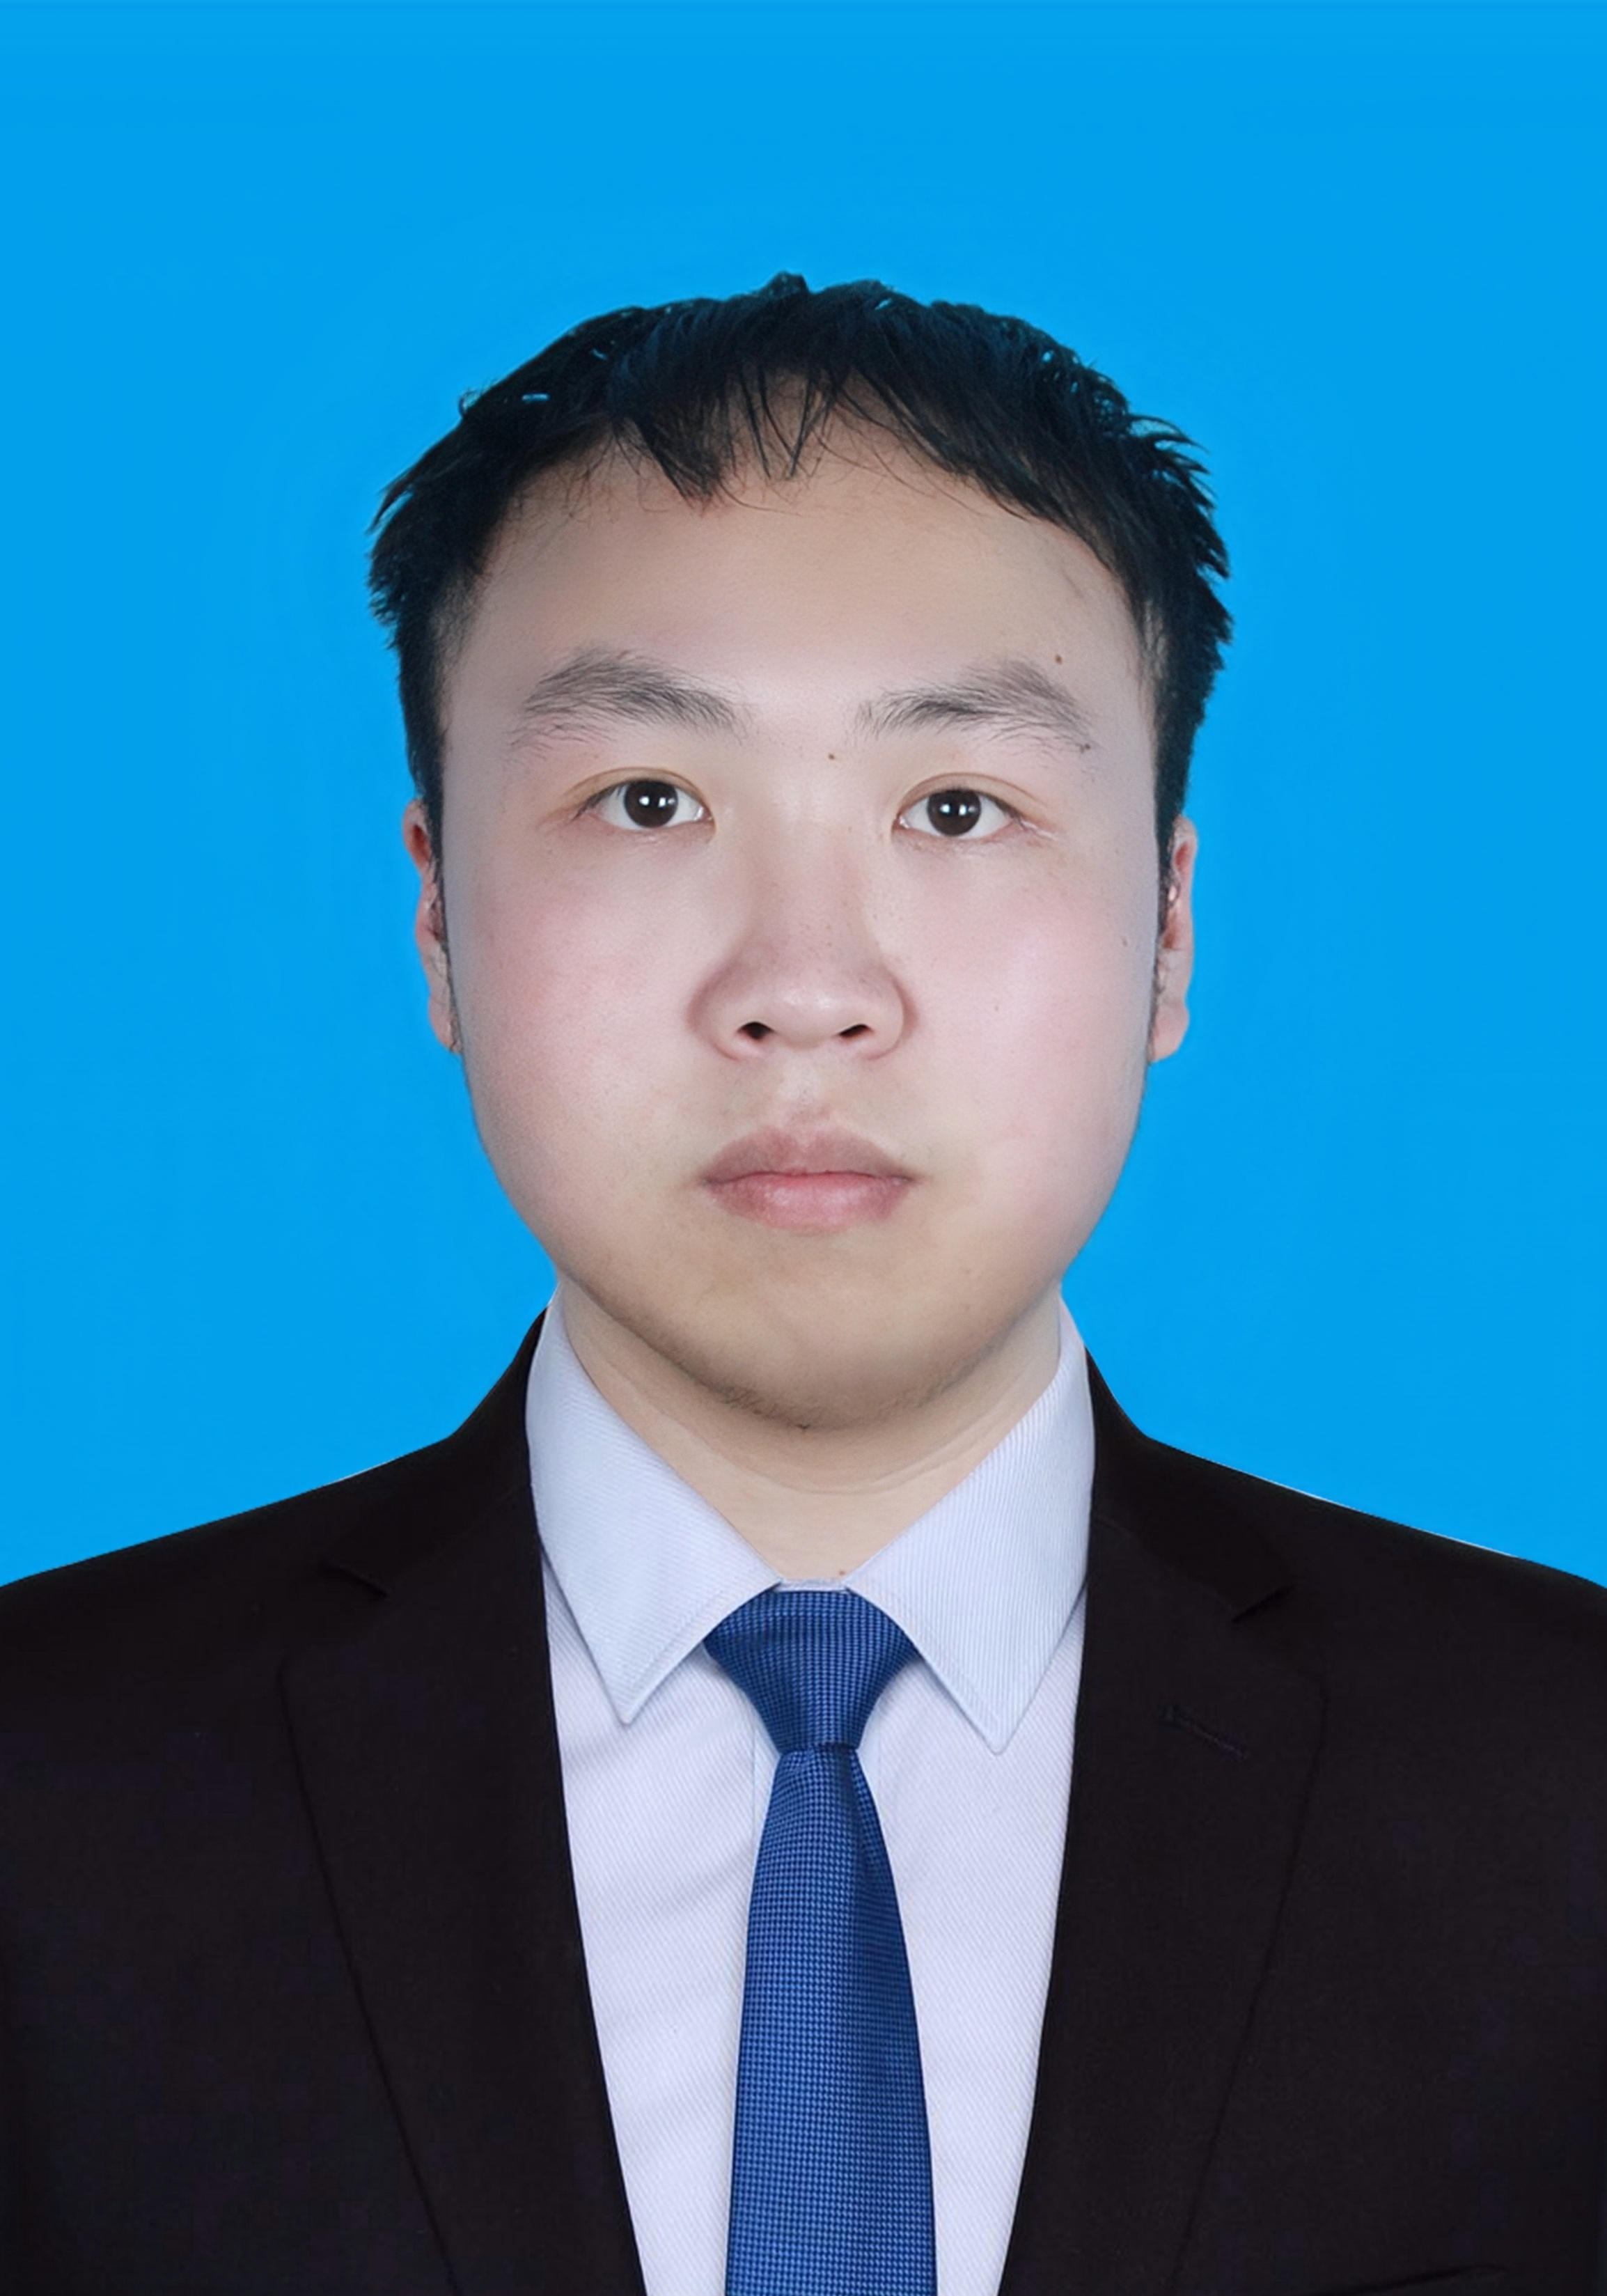
\includegraphics[width=2cm]{image.jpg}};
\end{tikzpicture}

\ResumeTitle

\section[教育经历]{教育经历}
\ResumeItem
[衡阳师范学院|硕士研究生]
{衡阳师范学院}
[\textnormal{电子信息,计算机学院|}  硕士研究生|师从李浪教授]
[2023.09—至今]

\ResumeItem
[长沙学院|本科生]
{长沙学院}
[\textnormal{机械设计制造及其自动化,机电工程学院|} 工学学士]
[2017.09—2021.06]

\section[技术能力]{技术能力\protect}
\begin{itemize}
  \item \textbf{语言}: 常用 C, Python, \LaTeX; 熟悉 Verilog, Assembly, \GrayText{Rust};了解 C$^{++}$, Java, \GrayText{TypeScript}。
  \item \textbf{工作流}: Linux, Shell, Vim, VsCode,  Git, GitHub。
\end{itemize}

% \section{工作经历}

% \ResumeItem{北京 ABCD 有限公司}
% [后端开发实习生/XXXX]
% [2020.10—2021.03]

% \begin{itemize}
%   \item \textbf{独立负责XXX业务后端的设计、开发、测试和部署。}通过 FaaS、Kafka 等平台实现站内信模板渲染服务。向上游提供 SDK 代码,增加或升级了多种离线和在线逻辑。完成了业务对站内信的多样需求。
%   \item \textbf{参与 XXX 的需求分析,系统技术方案设计;完成需求开发、灰度测试、上线和监控。}
% \end{itemize}
\section{论文发表\protect\footnote{本人一作,修改: \today}}

\ResumeItem{\textbf{Thread-Adaptive: Optimized Parallel Architectures of SLH-DSA on GPUs}}
[IEEE Transactions on Circuits and Systems II: Express Briefs (已完初稿,拟投), 2025]
\begin{itemize}
  \item 该论文为SLH-DSA后量子数字签名算法,提供高吞吐量异构实现方案。
\end{itemize}

\ResumeItem{\textbf{Low-Latency Implementation of Bitsliced SPN-Cipher on IoT Processors}}
[IEEE Transactions on Computers (一审中,CCF-A), 2025]
\begin{itemize}
  \item 该论文为SPN类结构对称加密算法,提供精简指令集上低延迟软件实现方案。
\end{itemize}

\ResumeItem{\textbf{Efficient implementations of CRAFT cipher for Internet of Things}}
[Computers and Electrical Engineering, 2024]
\begin{itemize}
  \item 该论文为CRAFT对称加密算法,提供高性能、高性价比和低成本硬件实现方案。
\end{itemize}

\section{项目经历}
\ResumeItem{主持湖南省研究生科研创新项目 ``轻量级分组密码的软硬件优化研究与实现''}
[项目编号:CX20240977]
[2024--至今]

\section{个人总结}

\begin{itemize}
  \item 性格: 本人乐观开朗、自驱能力强,具有较好的沟通能力和很强的团队合作精神。
  \item 研究展望:为理论安全的密码算法提供高性能和实现安全方案,继续从事密码工程学研究。
\end{itemize}

\end{document}
